We first describe how \livecodebench{} helps detect and avoid benchmark contamination in Section~\ref{subsec:contamination}. 
Next, we present the findings from our evaluations on \livecodebench{} in Section~\ref{subsec:model_comparisions}.

%discuss the performance of various models in Section~\ref{subsec:model_comparisions} and finally discuss results across scenarios in Section~\ref{subsec:scenario_specific_results}.


\subsubsection{Avoiding Contamination}
\label{subsec:contamination}
%A distinguishing aspect of our benchmark is the ability to evaluate models on problems released over different time windows.
%This allows us to measure the model performance on problems released after the cutoff date, thereby giving a performance estimate on \textit{unseen} problems.

\noindent \textbf{Contamination in \deepseek{} and \gptfouro{}.}
\livecodebench{} curates problems released since May $2023$. 
However, \deepseek{} was released Sep $2023$ and \gptfouro{}'s official cutoff date is Nov $2023$.
%models were released in Sep $2023$ and might have already been trained on some of the problems in our benchmark. 
%Similarly, \openai{} notes \gptfouro{} cutoff date in November. 
%\ag{some other models also released after may? maybe don't single out deepseek}
We can measure the performance of these models on the benchmark problems released after these dates, thereby estimating the performance of the model on previously unseen problems.
%As described in Section~\ref{sec:benchmark}, \livecodebench{} allows evaluating models on problems released over different time windows.
%Thus for a newly released model, we can evaluate it on the subset of problems released after the model's cutoff date.
%This allows us to measure uncontaminated model performance and thus offering fair comparisions.
%\livecodebench{} consists of problems released since May $2023$.
%therefore might be already trained on some of the problems in our benchmark.
Figure~\ref{fig:contamination_main} shows the performance of these models on \leetcode{} problems released in different months from May $2023$ and Aug $2024$. 
First, we notice stark drops in model performance --  \deepseekcodeB{33} model after Aug. $2023$, 
\gptfouro{} model after Nov. $2023$, 
\claudethrees{} model after Apr. $2023$.
%We notice a stark drop in the performance of \deepseekcodeB{33} model after Aug. $2023$ (right before its release date), 
These drops align with their release or cutoff dates which suggests that the earlier problems might indeed be contaminated.
This trend is consistent across other \livecodebench{} scenarios like repair and code execution, as depicted in Figure~\ref{fig:contamination_all_tasks_line}.
Concurrently, \citep{deepseek-coder} (Section 4.1, last paragraph) also acknowledge the possibility of \leetcode{} contamination, noting that ``\textit{models achieved higher scores in the LeetCode Contest held in July and August}''.
%Similarly, performance of the \gptfouro{} model drops on problems released since November (its official cutoff date).
% aligning with our findings.

%{\color{red} note contamination only in leetcode}
Interestingly, we find that this drop in performance primarily occurs for the \leetcode{} problems only and that the model performance is relatively smooth across the months for problems from other platforms. Figure~\ref{fig:atcoder_contamination} shows a relatively stable performance for all models on \atcoder{} problems.% released over different periods, with the possible exception of May and June. %\nj{update}

%Finally, we wish to point out that while the \deepseekcode{} models might be contaminated on the older problems, the models perform very well on problems released after the cutoff date and match or even outperform various strong baselines.

% like \claudetwo{} and \gptthreefiveturbo{}.

%show the performance of \deepseekcode{} models on the code generation task over time demonstrating a stark drop in performance after September 2023, highlighting the possible contamination.

%Finally, we would like to emphasize that \deepseekcode{} models extremely well on problems released post-contamination date, matching the performance of \gptthreefiveturbo{} model and is stronger than most other open access models.

\noindent \textbf{Performances of other models.}
We study performance variations in other models released more recently.
Particularly, \gptfourturbo{}, \mistrallarge{}, and \claudethrees{} models were released in Nov'$2023$, Feb'$2024$, and Mar'$2024$ respectively.
%Note that \gptfourturbo{} ($1106$-preview variant) and \claudethrees{} have cutoff dates April $2023$ and August $2023$ respectively.
Empirically, we do not observe significant performance variations across the months, as shown in Figure~\ref{app:fig:contamination_all_models}.%, particularly compared to the drops exhibited by the \deepseek{} models.
Interestingly, we find that even the \deepseekbaseB{33} model also suffers from contamination dropping from \passmetric{1} $\smallsim 60$ in May problems to \passmetric{1} $\smallsim 0$ in September \leetcode{} problems. 
%This also suggests the likely inclusion of competition problems in the pretraining of the \deepseek{} models, thereby affecting all instruction models trained from it.
Finally, \codestral{} achieves \passmetric{1} $36.5$ on problems released between May'23 and Jan'24 and \passmetric{1} $28.3$ on problems post Jan'24.


\begin{figure}[H]
  \centering
  \begin{minipage}[t]{0.49\textwidth}
    \centering
    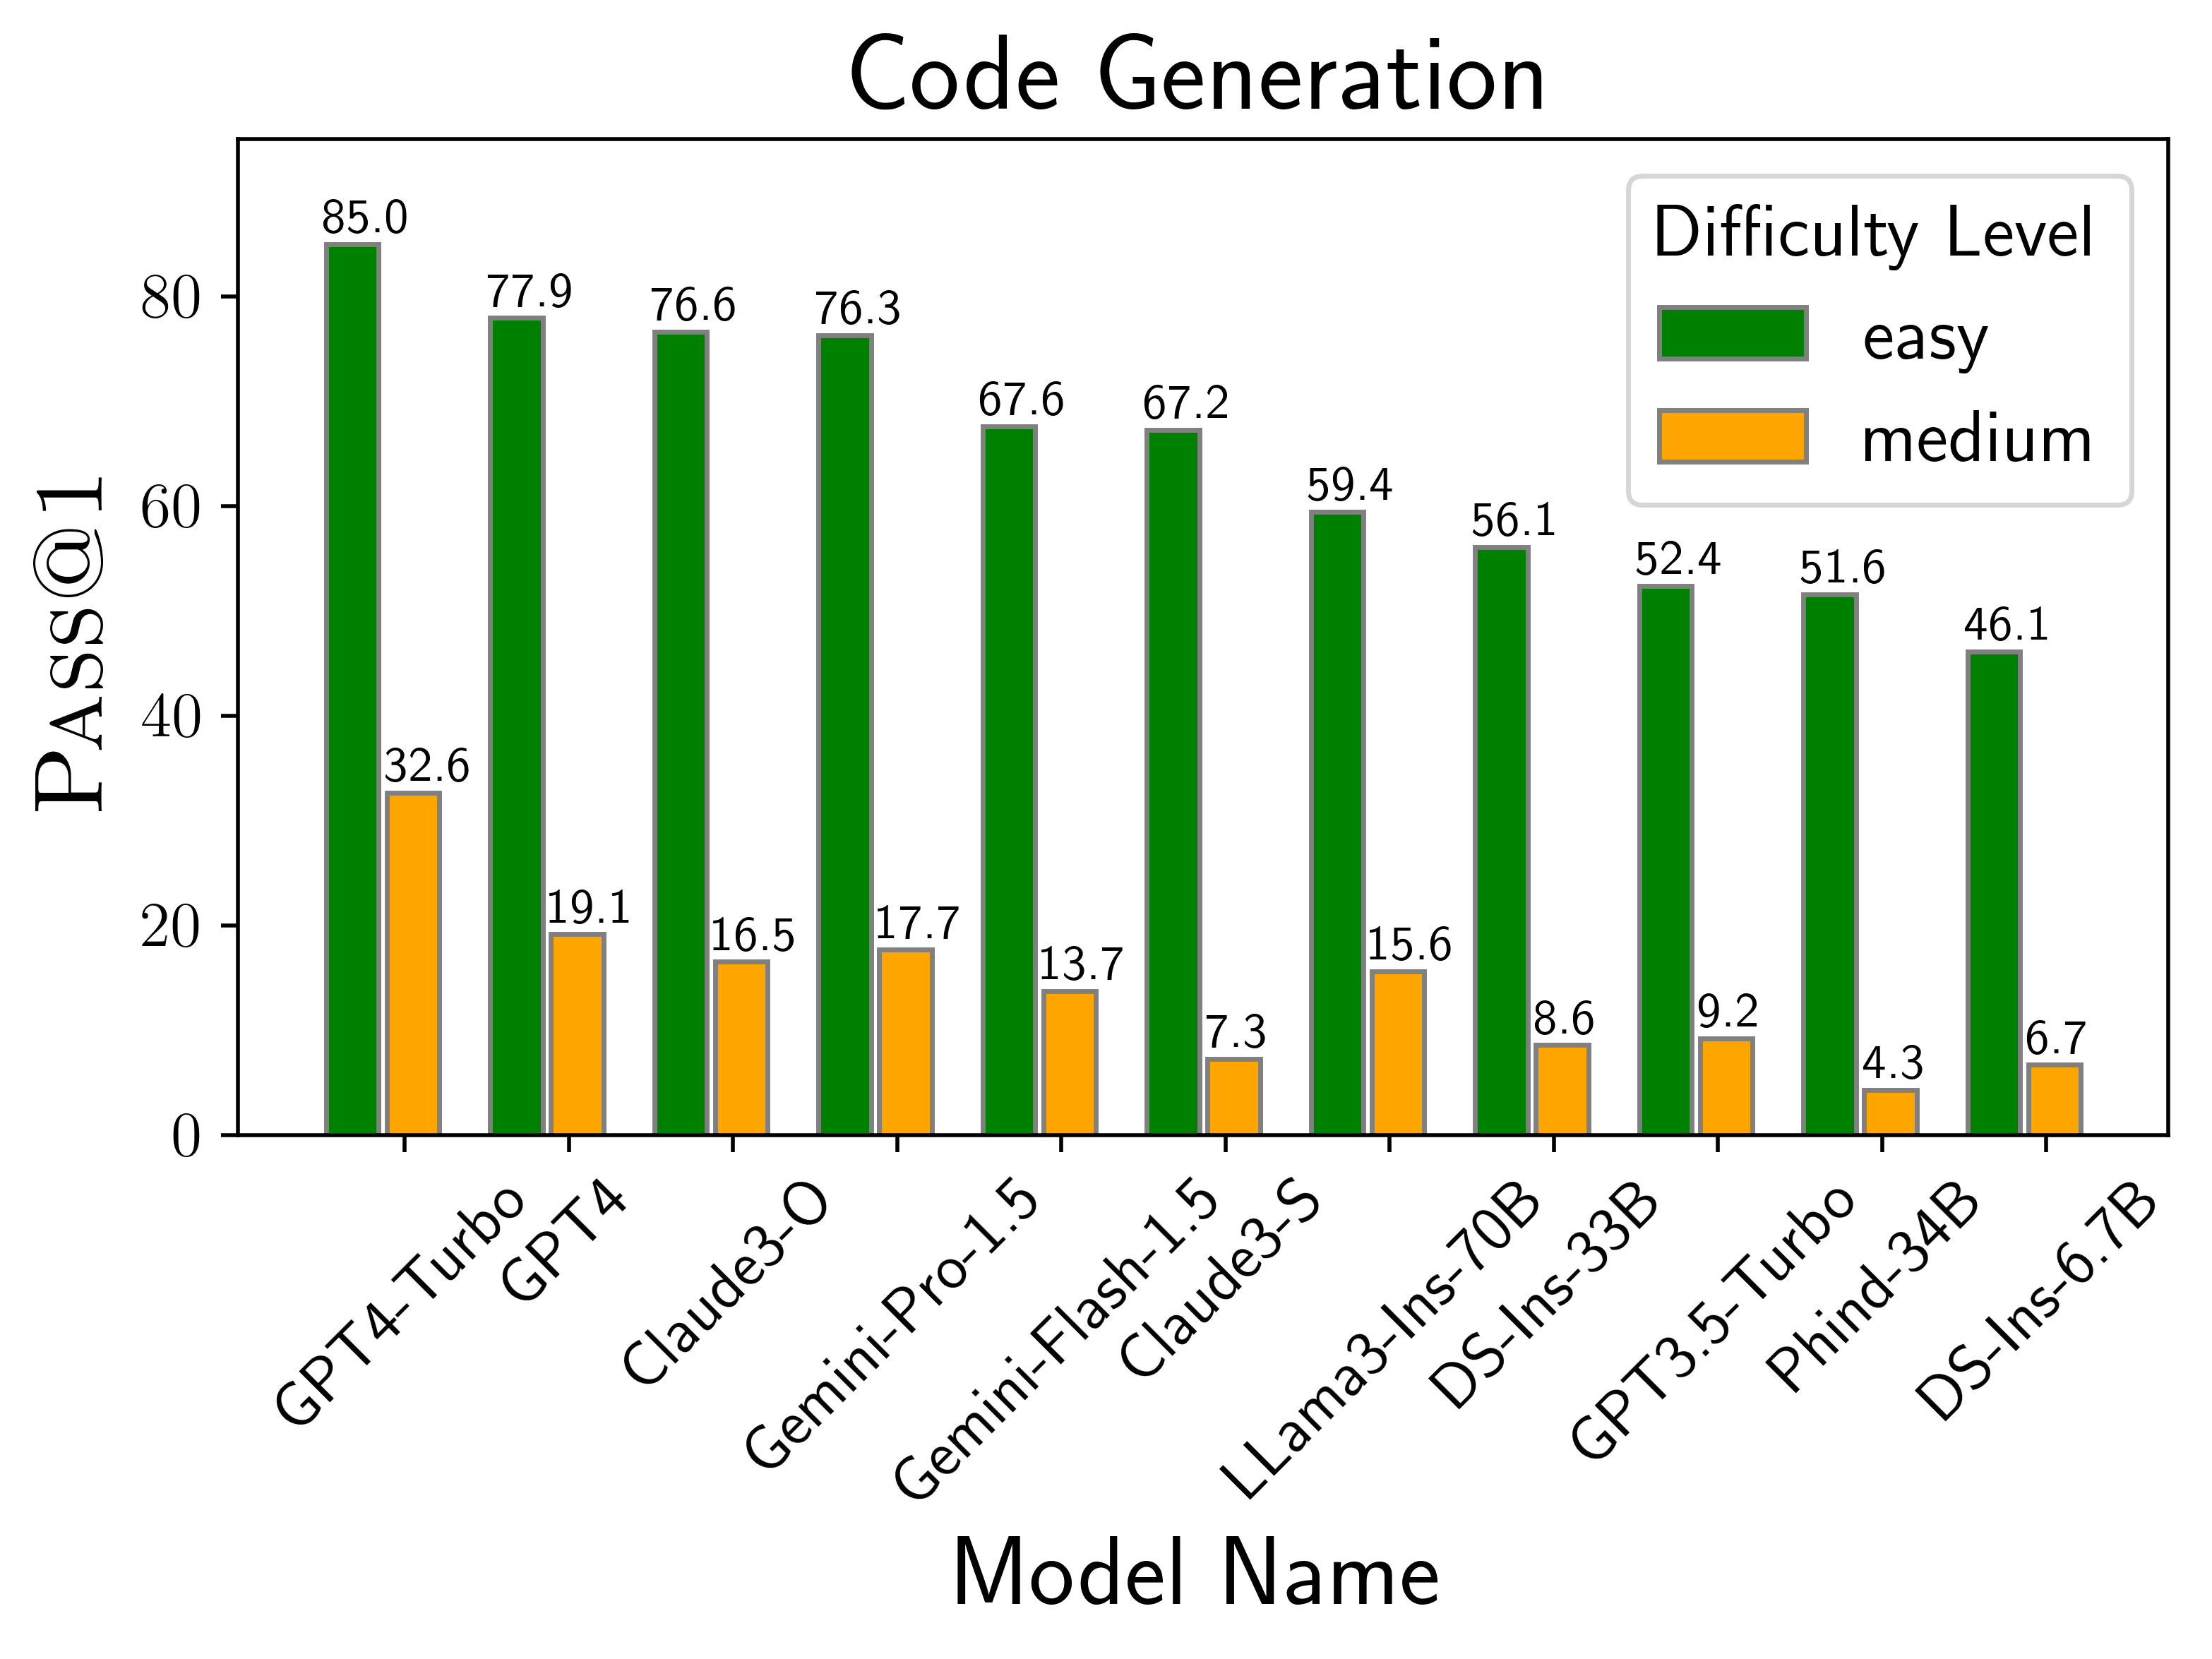
\includegraphics[width=\linewidth]{figures/main_results/codegen_performance.png}
  \end{minipage}\hfill
  \begin{minipage}[t]{0.49\textwidth}
    \centering
    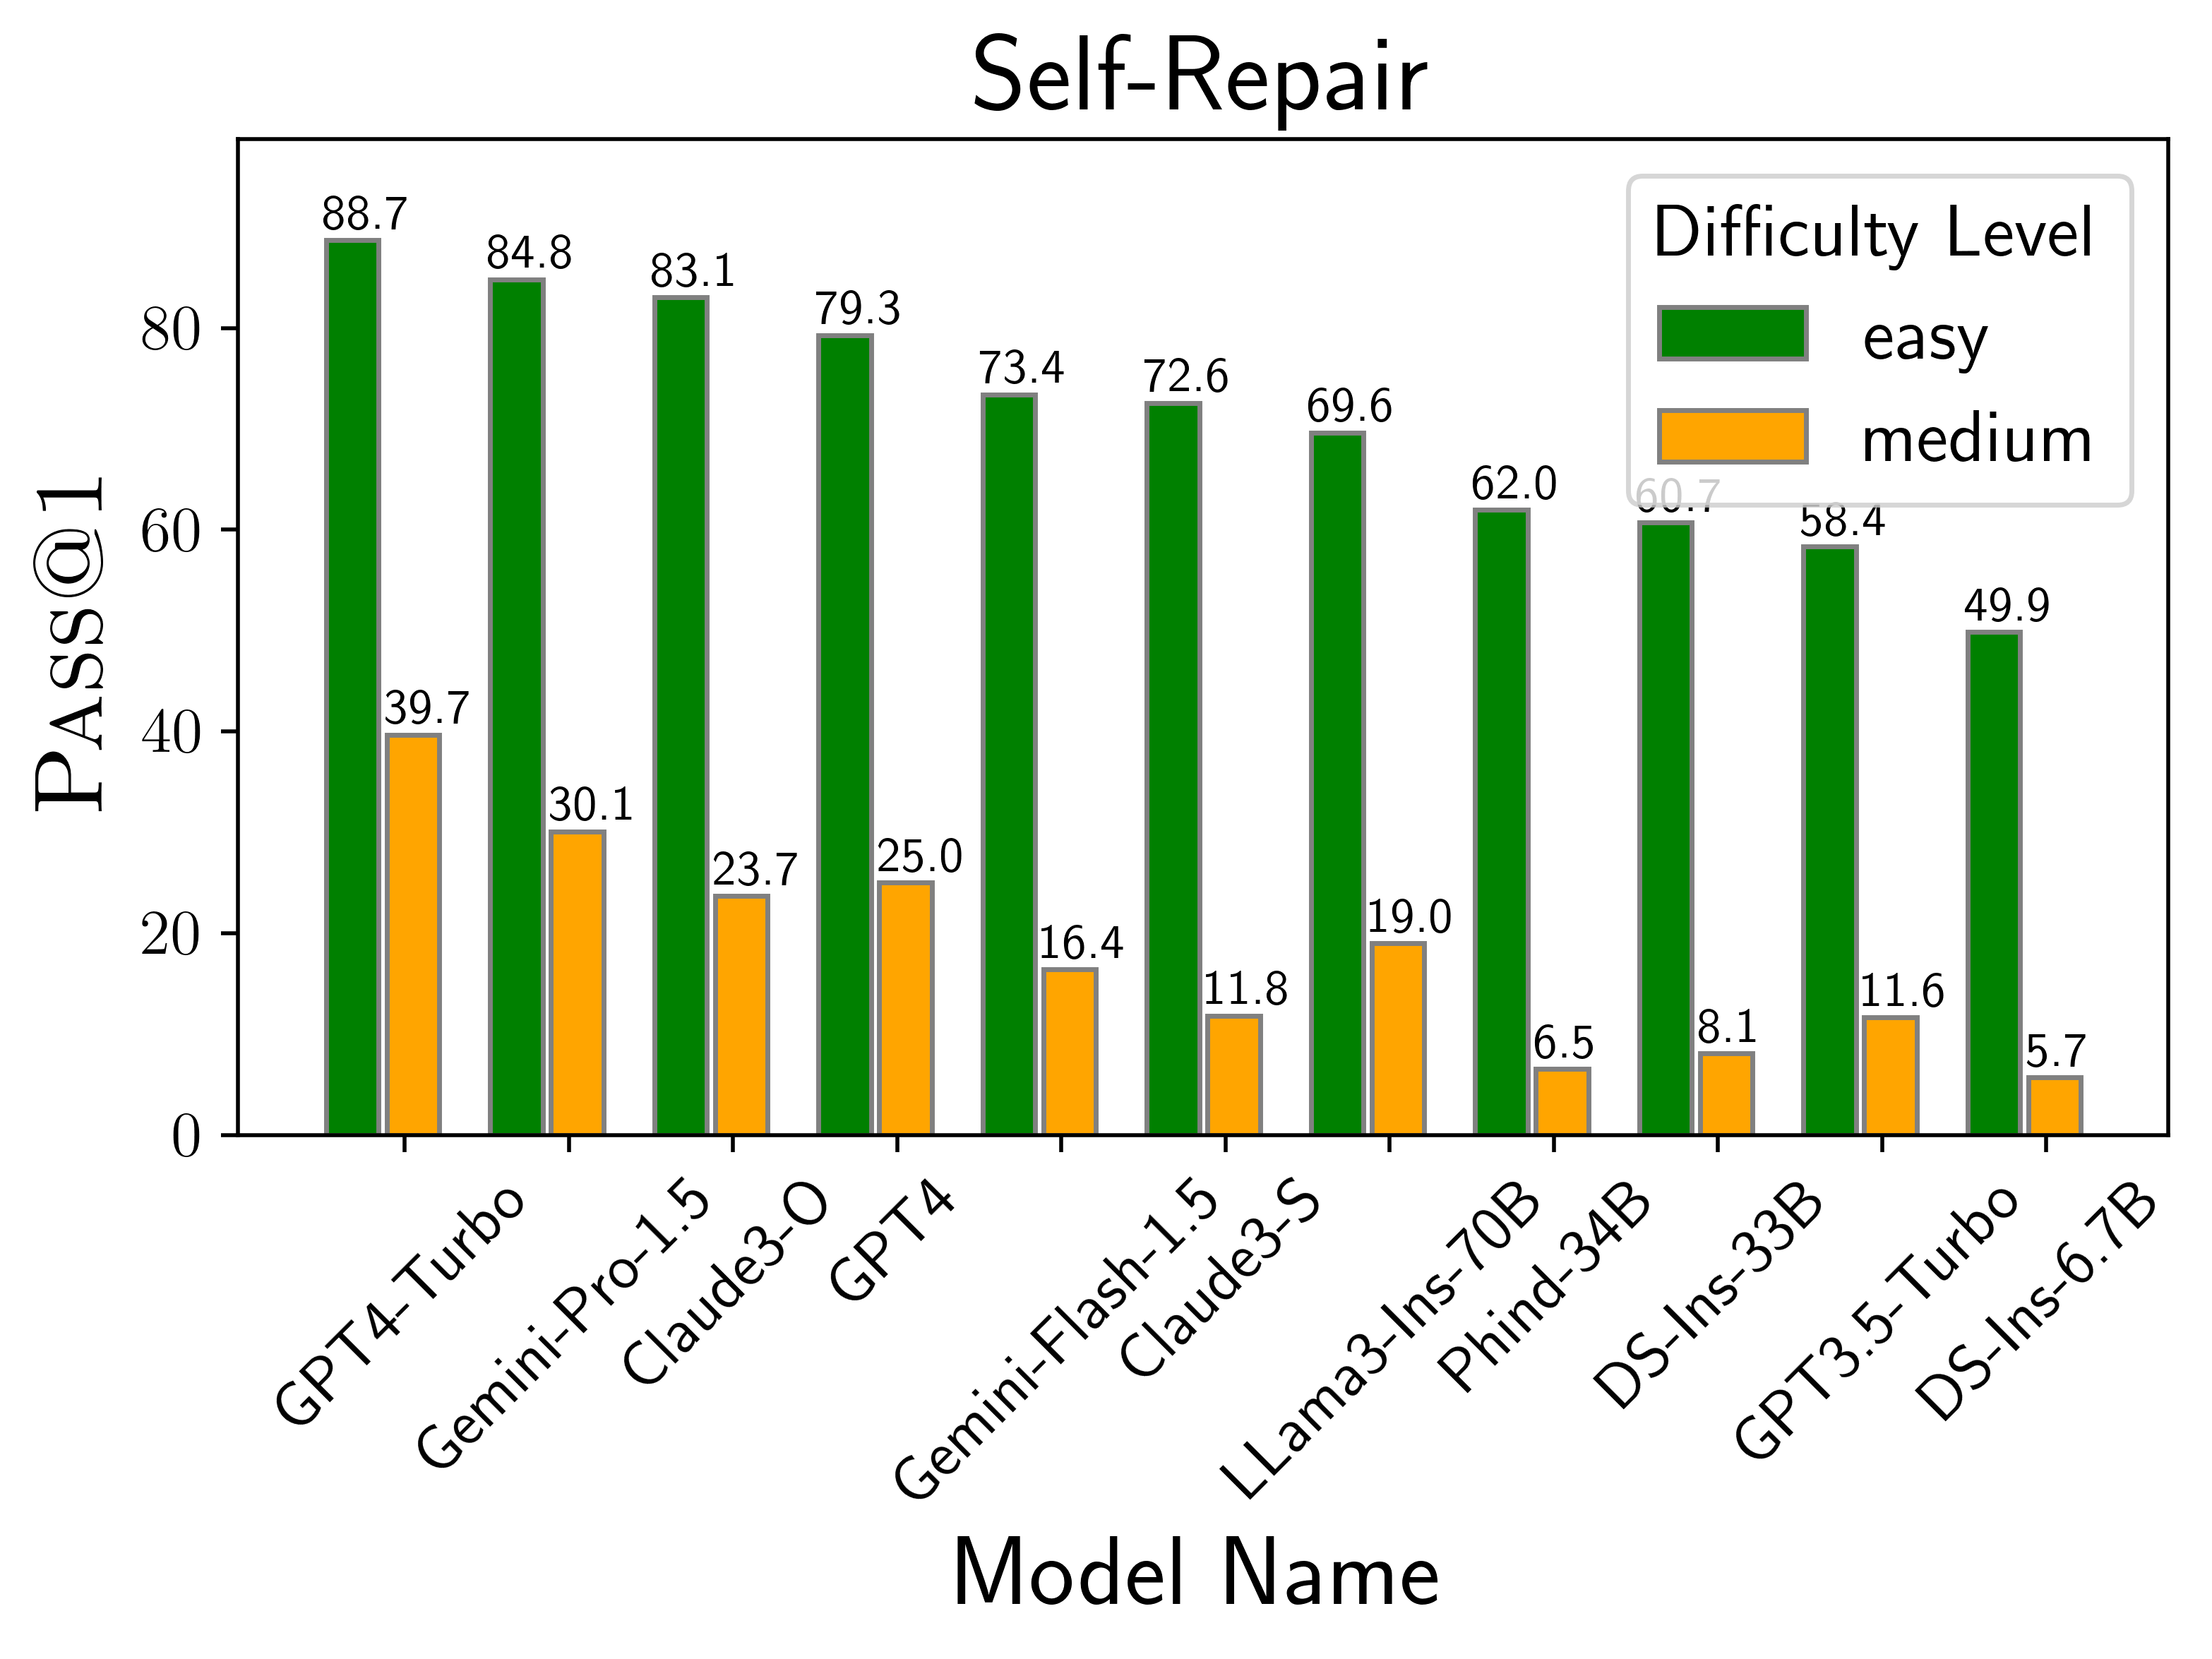
\includegraphics[width=\linewidth]{figures/main_results/repair_performance.png}
  \end{minipage}

  \vspace{0.5em}

  \begin{minipage}[t]{0.49\textwidth}
    \centering
    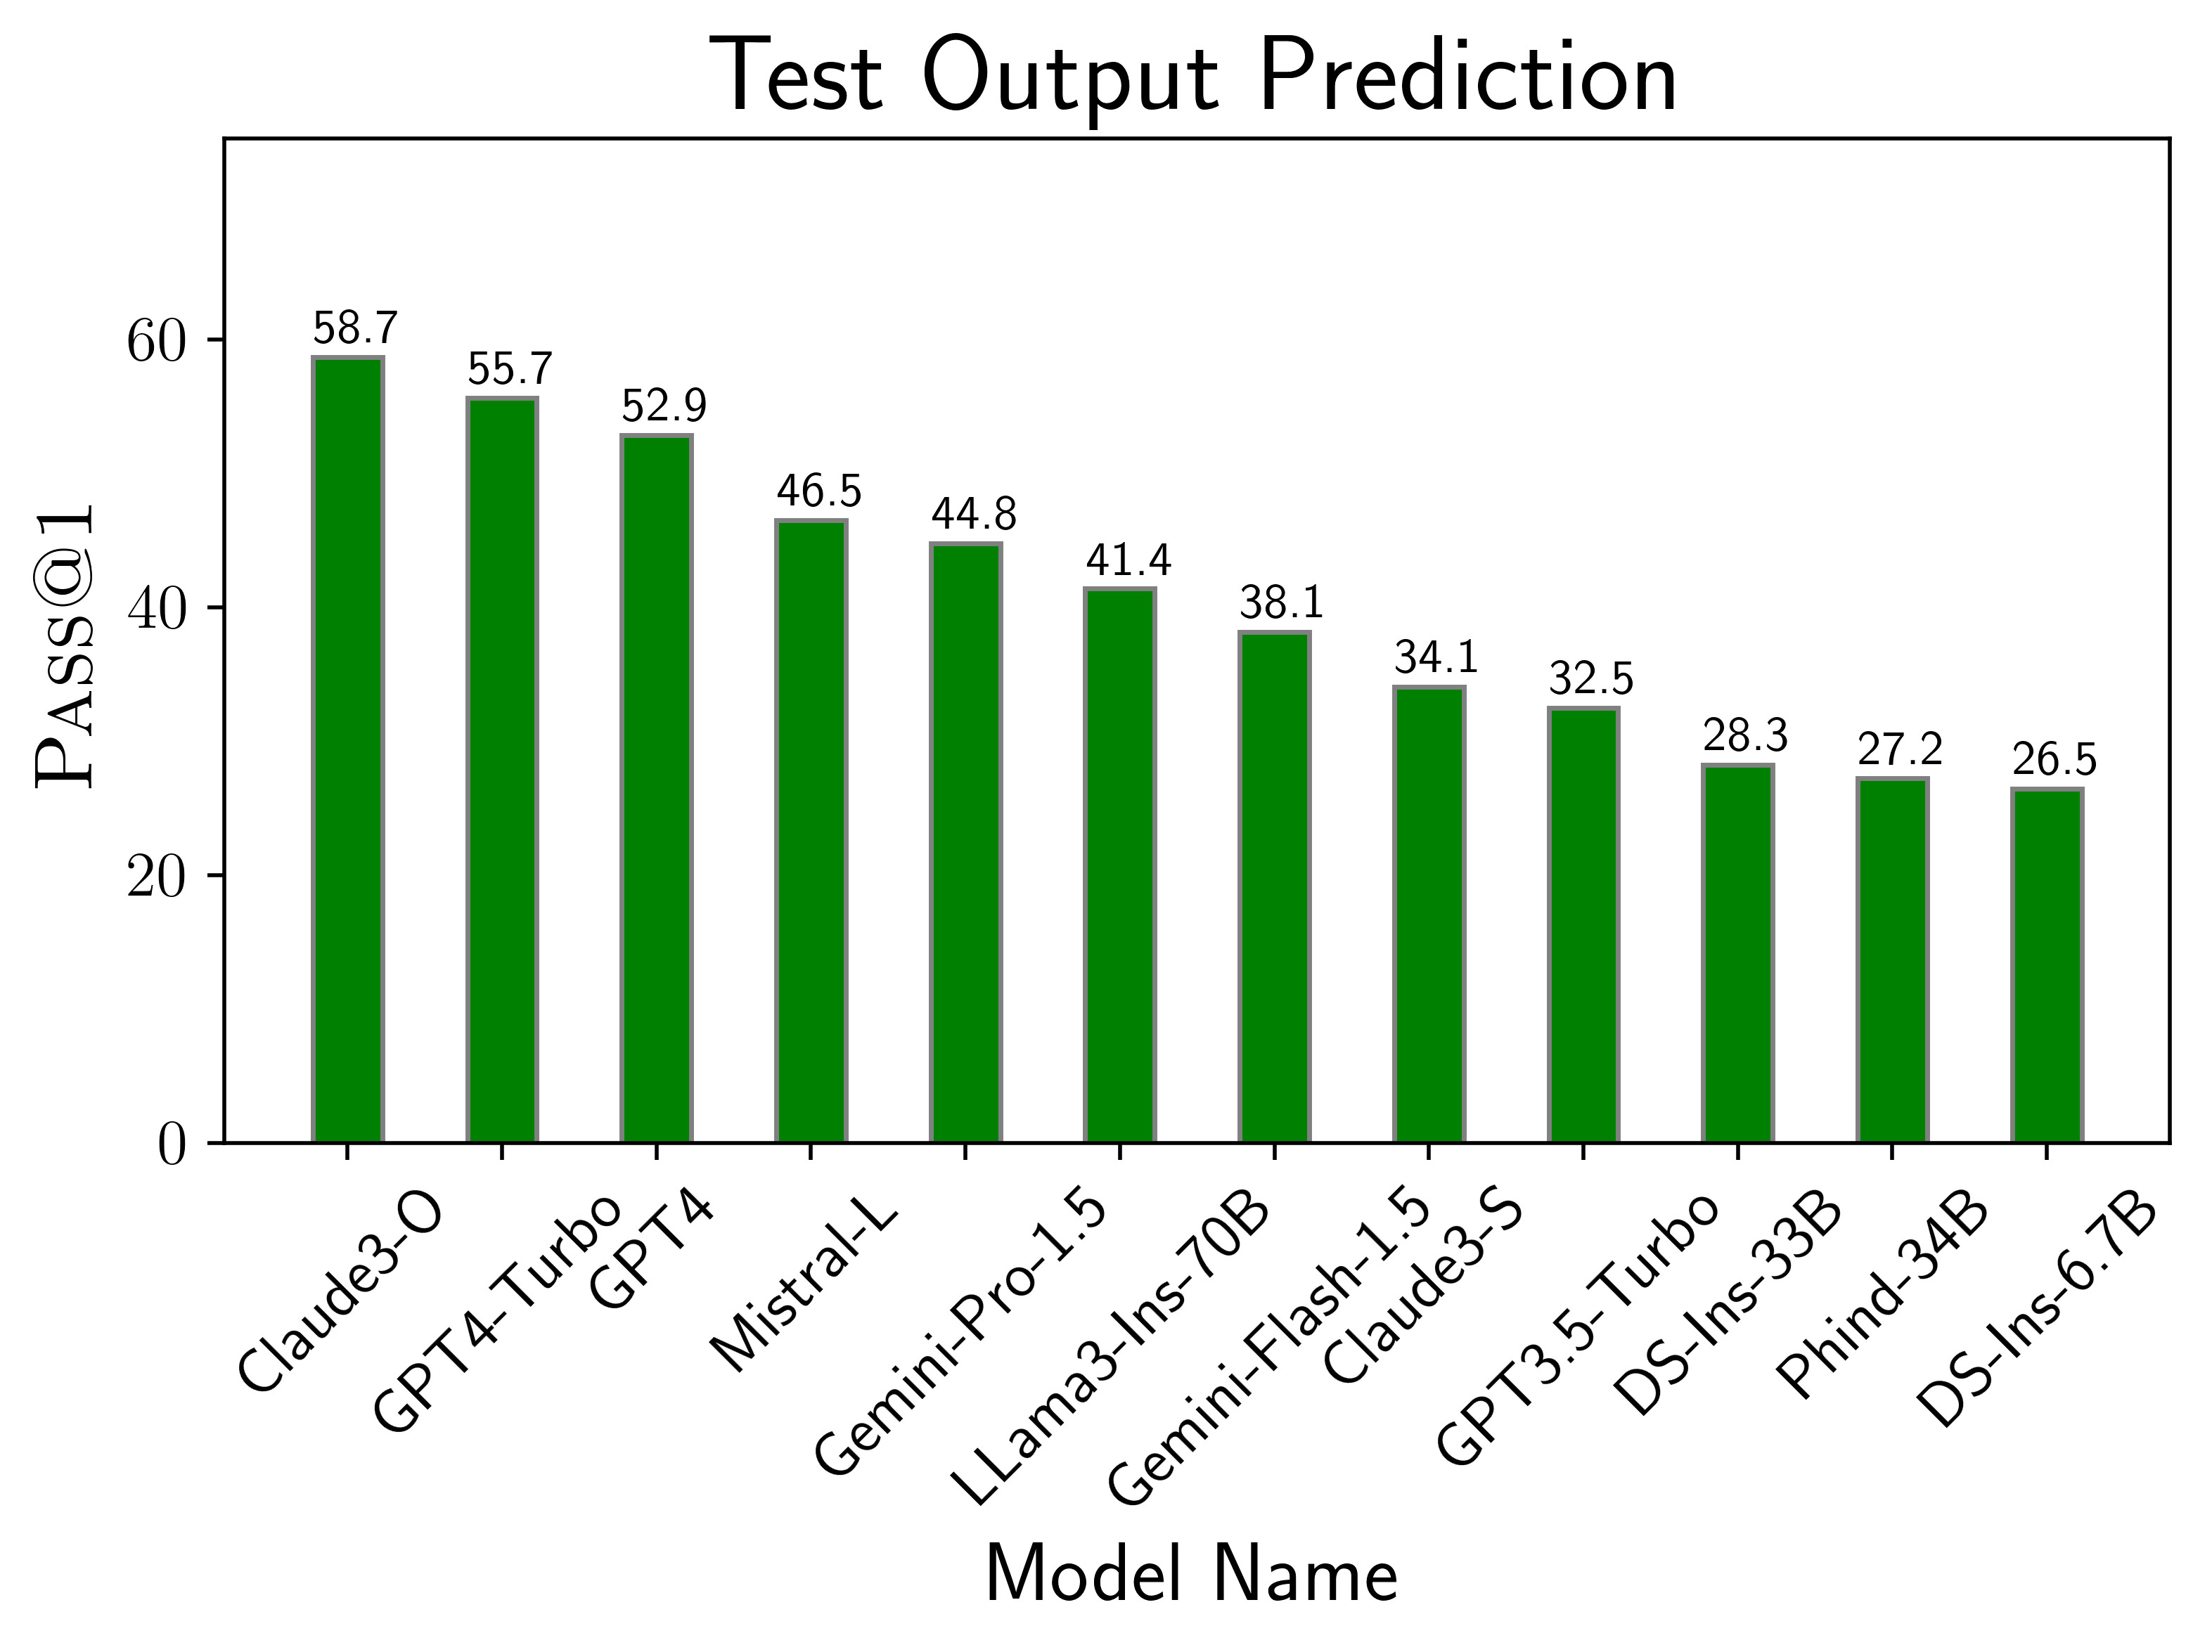
\includegraphics[width=\linewidth]{figures/main_results/testgen_performance.png}
  \end{minipage}\hfill
  \begin{minipage}[t]{0.49\textwidth}
    \centering
    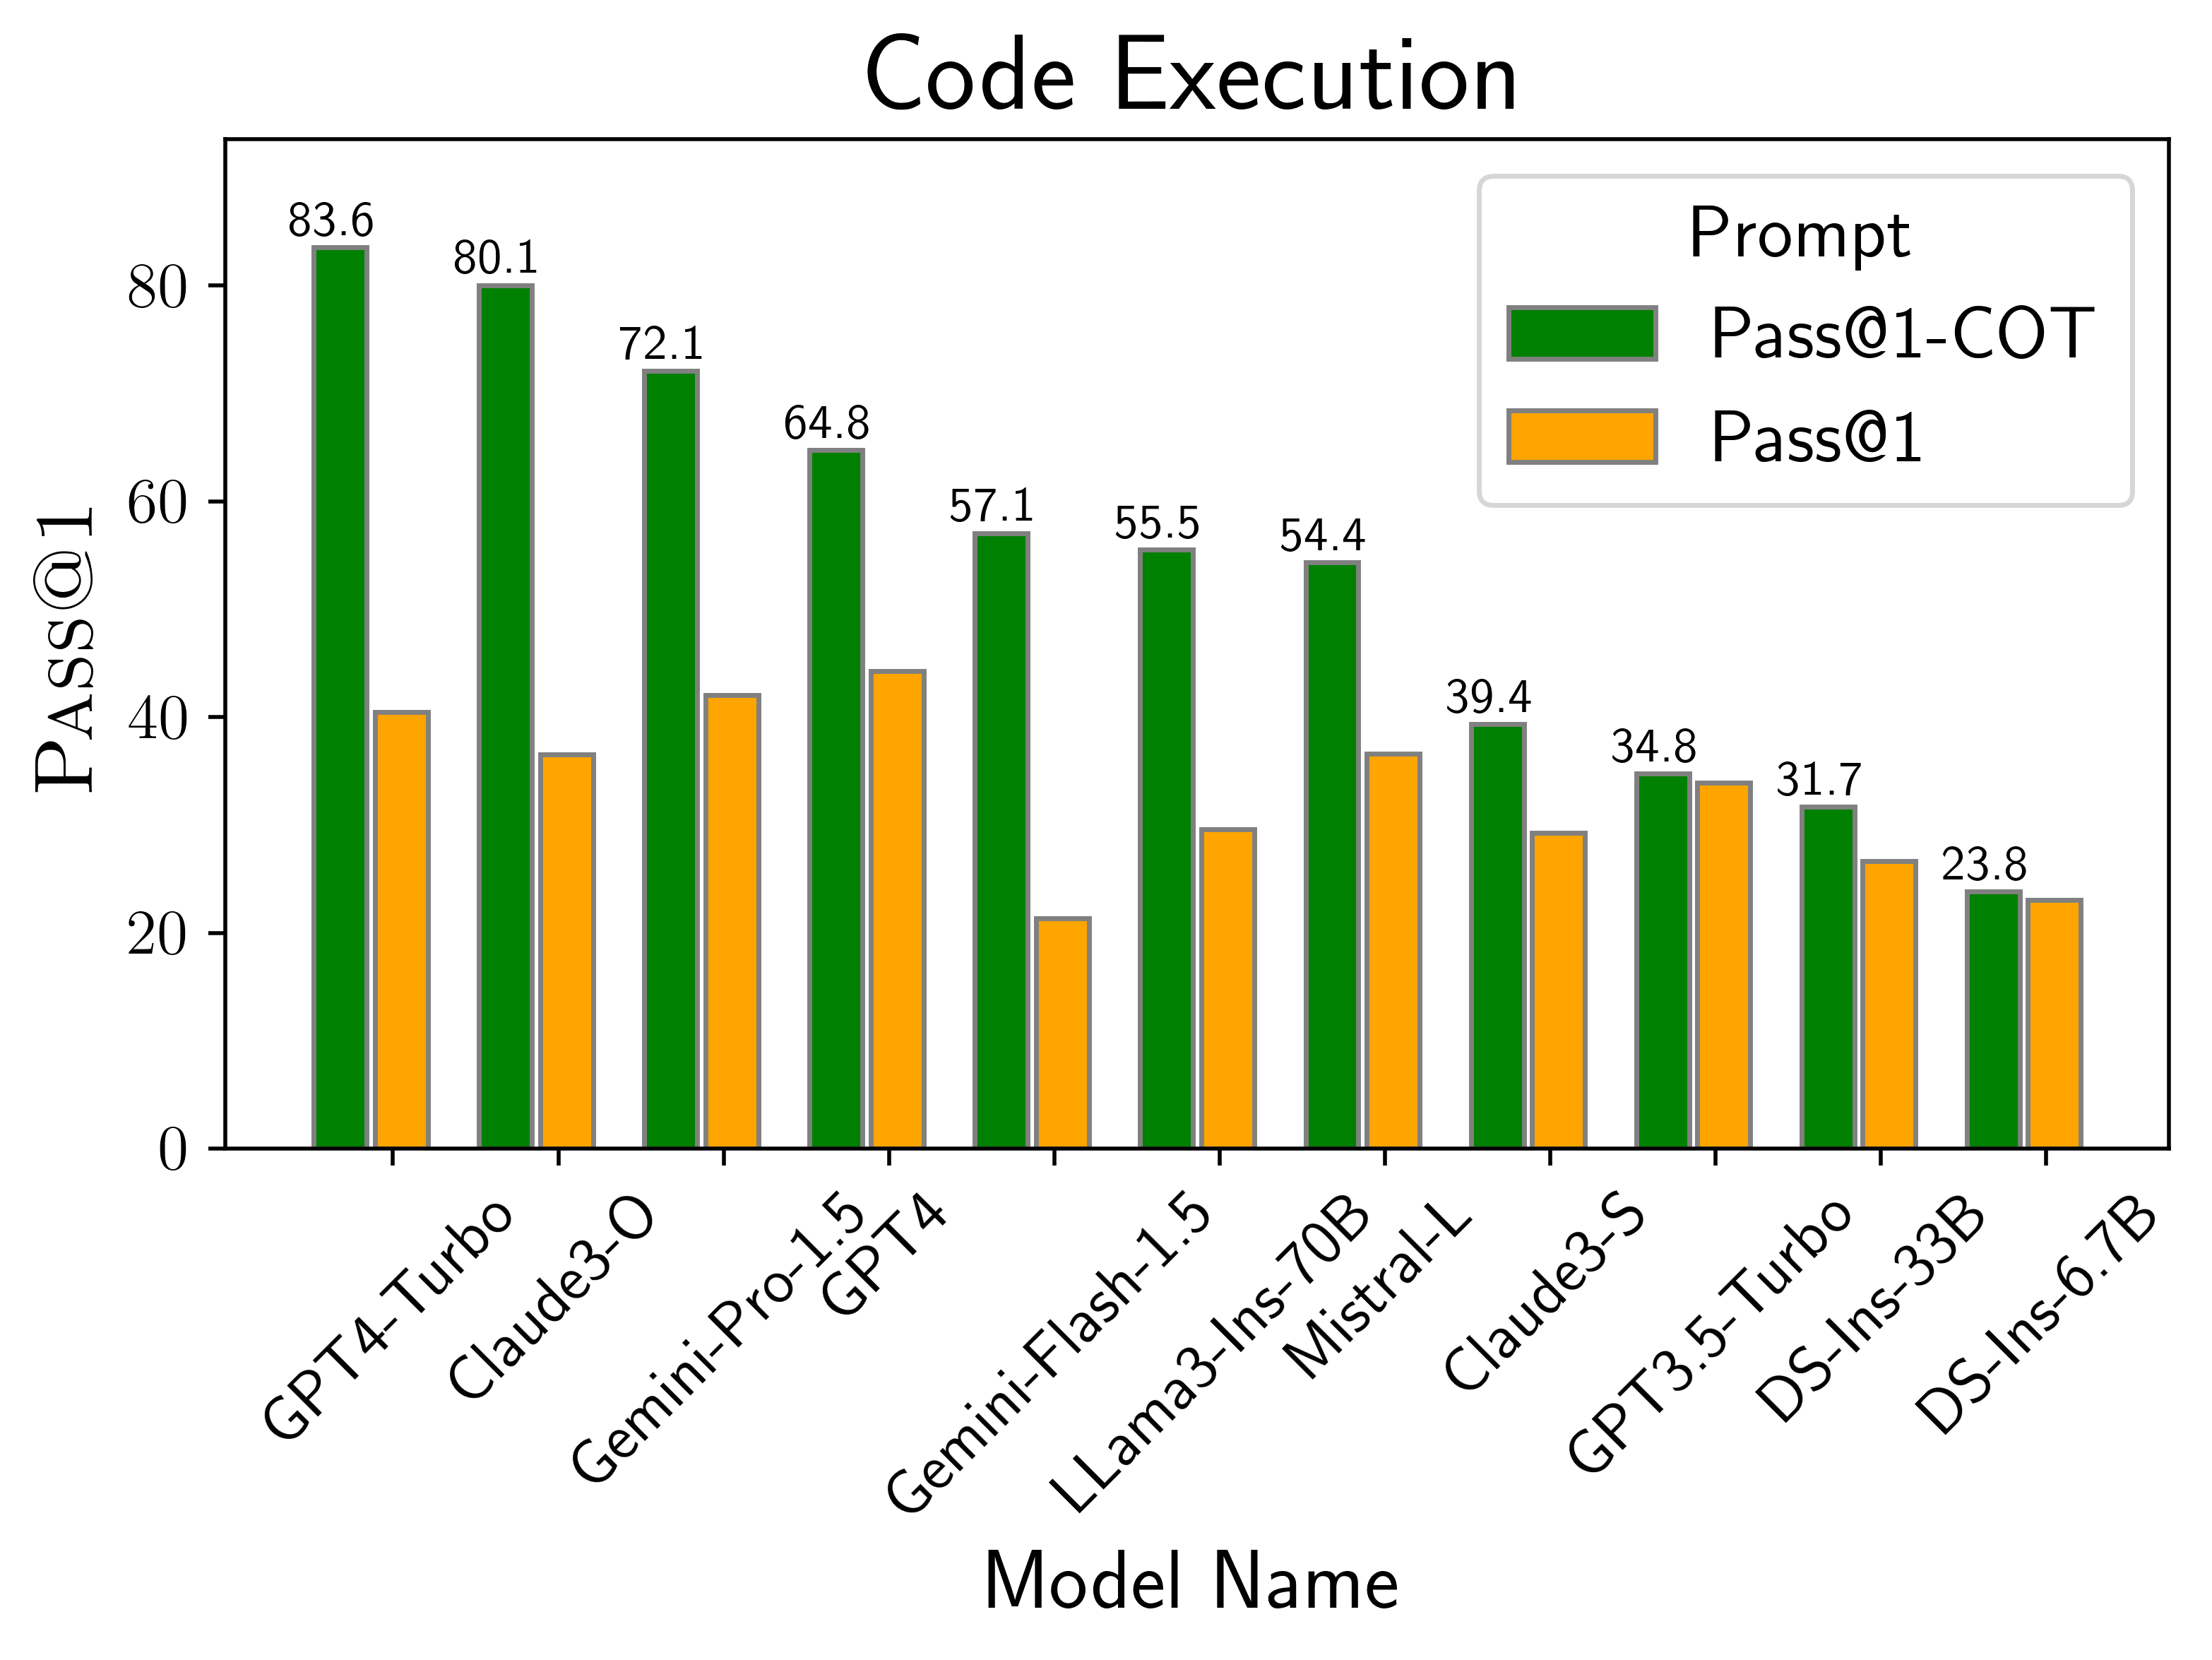
\includegraphics[width=\linewidth]{figures/main_results/execution_performance.png}
  \end{minipage}

  \caption{Model performances across the four scenarios available in \livecodebench{}.}
  \label{fig:results_plots}
\end{figure}
  



\subsubsection{Performance and Model Comparisons}
\label{subsec:model_comparisions}
We provide our model comparison findings here (and in Appendix~\ref{app:sec:results}).
%We evaluate $34$ instruction-tuned models (and $18$ base models used in the code generation scenario) on \livecodebench{}.
%These models range from closed access to open access with their various fine-tuned variants.
To overcome contamination issues in \deepseek{} models, we only consider problems released since Sep $2023$ for all evaluations below.
Figure~\ref{fig:results_plots} shows the performance of a subset of models across the four scenarios. 
% We highlight our key findings below.


\noindent \textbf{Holistic Evaluations.}
We have evaluated the models across the four scenarios currently available in \livecodebench{}.
Figure~\ref{fig:contamination_main} displays the performance of models on all scenarios along the axes of the polar chart.
First, we observe that the relative order of models remains mostly consistent across the scenarios.
This is also supported by high correlations between \passmetric{1} metric across the scenarios -- 
over $0.88$ across all pairs as shown in Figure~\ref{app:fig:correlation_matrix}.
%Interestingly, the correlations are larger for related tasks, $0.98$ for generation and self-repair, and $0.96$ for test output prediction and code execution. 
%This correlation drops to $0.89$ for generation and execution scenarios.
However, despite the strong correlation, the relative differences in performance do vary across the scenarios.
For example, \gptfourturbo{} further gains performance gap over \gptfour{} in the self-repair scenario after already leading in the code generation scenario.
Similarly, \claudeopus{} and \mistrallarge{} perform well in tasks involving \chainot{}, particularly in the code execution and test output prediction scenarios.
For instance, \claudeopus{} even outperforms \gptfourturbo{} in the test output prediction scenario.
%Similarly, \mistrallarge{} outperforms \claudesonnet{} in both scenarios after trailing behind in code generation and repair scenarios.
These differences highlight the need for holistic evaluations beyond measuring code generation capabilities.

%Similarly, the difference in performance between \gptfourturbo{} and \gptfour{} becomes even more pronounced in the 
%code execution scenario highlighting the benefit of holistic evaluations.
%difference between strongest models becomes more pronounced in self-repair where \gptfourturbo{} further overshawdows \gptfour{}.


\noindent \textbf{Comparison to \humaneval{}.}
Next, we compare how code generation performance metrics translate between \livecodebench{} and \humaneval{}, 
the primary benchmark used for evaluating coding capabilities.
Note that we use \humanevalplus{} providing more accurate evaluations.
Figure~\ref{fig:he_vs_lcb} shows a scatter plot of \passmetric{1} on \humanevalplus{} versus \lcb{}-Easy code generation scenario. 
We find only a moderate correlation of $0.72$, with much larger performance variations on \lcb{}-Easy.
%\redo{(ranging from $16.9$ to $85.0$), while \humanevalplus{} shows a smaller range ($50.6$ to $81.3$)}.
% Thus \livecodebench{} allows better discrimination between models.

Additionally, we observe that the models cluster into two groups, shaded in red and green.
The models in the green-shaded region lie close to the $x=y$ line, indicating that they perform similarly on both benchmarks.
On the other hand, models in the red shaded region  perform well  on \humanevalplus{} but not as well on \livecodebench{}.
Interestingly, the green-shaded cluster contains base models or closed-access models, 
while the red-shaded cluster primarily comprises fine-tuned variants of open-access models.
The well-separated clusters suggest that many models that perform well on \humaneval{} might be overfitting on the benchmark, and their performances do not translate well to problems from other domains or difficulty levels like those present in \livecodebench{}. %\nj{update}
\begin{figure}[!t]
    \centering
    \includegraphics[width=0.99\textwidth]{figures/main_results/lcb_vs_he.png}
  \vspace{-3pt}
    \caption{
        Scatter plot comparing \passmetric{1} of models on \humanevalplus{} versus \lcb{}-Easy{} (time-window Sep $2023$ to May $2024$).
        The green-shaded region marks models with aligned performance across benchmarks, while the red-shaded region marks models with much stronger performance on \humanevalplus{}.
    }

        \label{fig:he_vs_lcb}
        \vspace{-15pt}
\end{figure}

%This highlights two key findings: (a.) \livecodebench{} problems allow for better discrimination between models, and (b.) models that perform well on \humaneval{} might be overfitting on the benchmark, and their performances do not translate well to problems from other domains or difficulty levels.
%\ag{we discussed this claim on slack}
Indeed, \humaneval{} has small and isolated programming problems and thus easier to overfit.
In contrast, \livecodebench{} problems are sourced from reputable coding platforms offering more challenging problems with higher diversity and difficulty levels.
We detail instances of this overfitting (\deepseekcodeB{1.3}, \deepseekcodeB{6.7}, and \codeqwen{}) in Figure~\ref{fig:he_vs_lcb} caption.
%This potential overfitting is particularly exemplified by \deepseekcodeB{1.3} which achieves $59.8$\% \passmetric{1} on \humanevalplus{} but only $26.3$\% on \lcb{}-Easy.
% Thus, while it boasts better performance compared with \geminipro{} and \claudeinstantone{} on \humanevalplus{}, it performs considerably worse on \lcb{}-Easy.
% Similarly, \codeqwen{}, \deepseekcodeB{6.7}, and \magicoder{6.7} perform better than \mistrallarge{}, \claudetwo{}, and \claudesonnet{} on \humanevalplus{} but are considerably worse on \lcb{}-Easy.% \nj{modify to codeqwen?}

%For instance, \deepseekcodeB{1.3} which achieves $59.8$\% \passmetric{1} on \humaneval{}, but only $29.2$\% the \passmetric{1} on \livecodebench{} easy subset. 
%\gptfour{} model in contrast achieves close to $80$\% \passmetric{1} on both \humaneval{} and \lcb{}-Easy highlighting likely close difficulty level between the two benchmarks. \ag{hmm a bit careful with wording here, people think humaneval is contaminated}
%Finally, we wish to highlight that \livecodebench{} provides a good evaluation set, allowing for discrimination while avoiding contamination and overfitting.
%In contrast, \livecodebench{} problems mimic more real-world and algorithmic coding problems, and the ability to generalize and do well on them would imply software engineer proficiency.
%Thus while many models claim similar or better performance than \gptfour{}, we find that such claims need to be taken with a grain of salt.


% \noindent \textbf{Highlighting the gap between SoTA and open models.} 
% %\ag{instead of "vacuum beyond", maybe "highlighting the gap between gpt4 and open"? i think the cool thing to advertise is that our benchmark can actually differentiate gpt4 unlike HE} -- totally agreed, was going for that vibe
% One distinct observation from our evaluations is the large gap between SoTA models and open models across all scenarios.
% Particularly, \gptfourturbo{}, \gptfour{}, \geminiproonefive{} and \claudeopus{} lead across the benchmarks with wide performance margins over other models.
% This distinguishes \livecodebench{} from prior benchmarks (like \humaneval{}) where various open models have achieved similar or better performance. 
% For example, \deepseekcodeB{33} is merely $4.3$ point behind \gptfourturbo{} on \humanevalplus{} but 
% $16.2$ points ($69$\%) on \lcb{} code generation scenario.
% This gap either holds or sometimes even amplifies across other scenarios.
% For instance, consider test output prediction and code execution (with \chainot{}) where \gptfourturbo{} leads the \deepseekcodeB{33} model by $96\%$ and $134\%$ respectively!
% %This gap is only amplified by \gptfourturbo{} which further improves over \gptfour{} across all tasks (only with \chainot{} for code execution). 
% %\ag{could say a bit more for the other tasks}

% We qualitatively analyze code samples generated by the leading model, \gptfourturbo{}, and find that it generates more readable code.
% Specifically, the code consists of more inline natural language comments that \textit{reason} or \textit{plan} before producing the code.
% (see Figure~\ref{fig:gptfouroutput}).
%Interestingly, we observe that apart from improved performance, the new model generates more readable code with inline comments that \textit{plan} the code generation process. 
% We verify this quantitatively and find \gptfourturbo{} generated uses $19.5\times$ more comment tokens compared to \gptfour{}.


%\ag{for this point and the point after, good to clarify which scenarios you're referring to (all?)}
\noindent \textbf{Comparing Base Models.}
We use four families of base models and compare them on the code generation scenario.
A one-shot prompt is used for all models to avoid any formatting and answer extraction issues.
We find \llamabase{} and \deepseekcode{} models are significantly better than both \cllama{} and \starcodertwo{} base models with 
a \deepseekbaseB{6.7} model even outperforming both \cllamabaseB{34} and \sctwobaseB{15} models.
% Next, we observe that \sctwobaseB{15} also outperforms the \cllamabaseB{34} model (similiar to findings in ~\cite{starcoder2}).
Note that some \lcb{} specific differences can potentially be attributed to data curation approaches.
For instance, \smalltextsc{SC} models (and potentially \smalltextsc{DS} as discussed in Section~\ref{subsec:contamination}) use competition problems during pre-training.% highlighting the need for diverse and clean data for training code \llms{}.
%Similarly, training methodologies (like epochs and learning schedules) can also play a role in the difference and
%we leave a thorough investigation of this for future work. \nj{add llama3}


\noindent \textbf{Role of Post Training.}
Post-training improves performance on both \humanevalplus{} and \livecodebench{} for the code generation scenario.
Particularly, on \lcb{} \llamaB{70}, \deepseekcodeB{33} and \phind{} improve \passmetric{1} over their base models by $8.2$, $7.3$ and $9.5$ points respectively.
% Similar gains are observed in previous benchmarks (like \humanevalplus{}) as well highlighting necessity
This highlights the importance of good post-training datasets  for building strong \llms{}. 
%Thus, even though fine-tuning is assumed to not significantly alter model capabilities,
%it is essential for improving performance by eliciting the right model behavior. \nj{add llama3 etc}
At the same time, we note that the base models have \textit{aligned} performances on \lcb{} code generation and \humanevalplus{} benchmarks and lie within or close to the green shaded region in Figure~\ref{fig:he_vs_lcb}.
However, the fine-tuned open models exhibit a larger performance gap, with much better performances on \humanevalplus{}.
On the other hand, the closed-access models are still aligned across both benchmarks.
This suggests the necessity of more diverse post-training data mixtures. 
% that the fine-tuning data for open models might not be as diverse as that for closed models, leading to a lack of generalization to different kinds of problems.


\begin{figure}[!t]
    \centering
    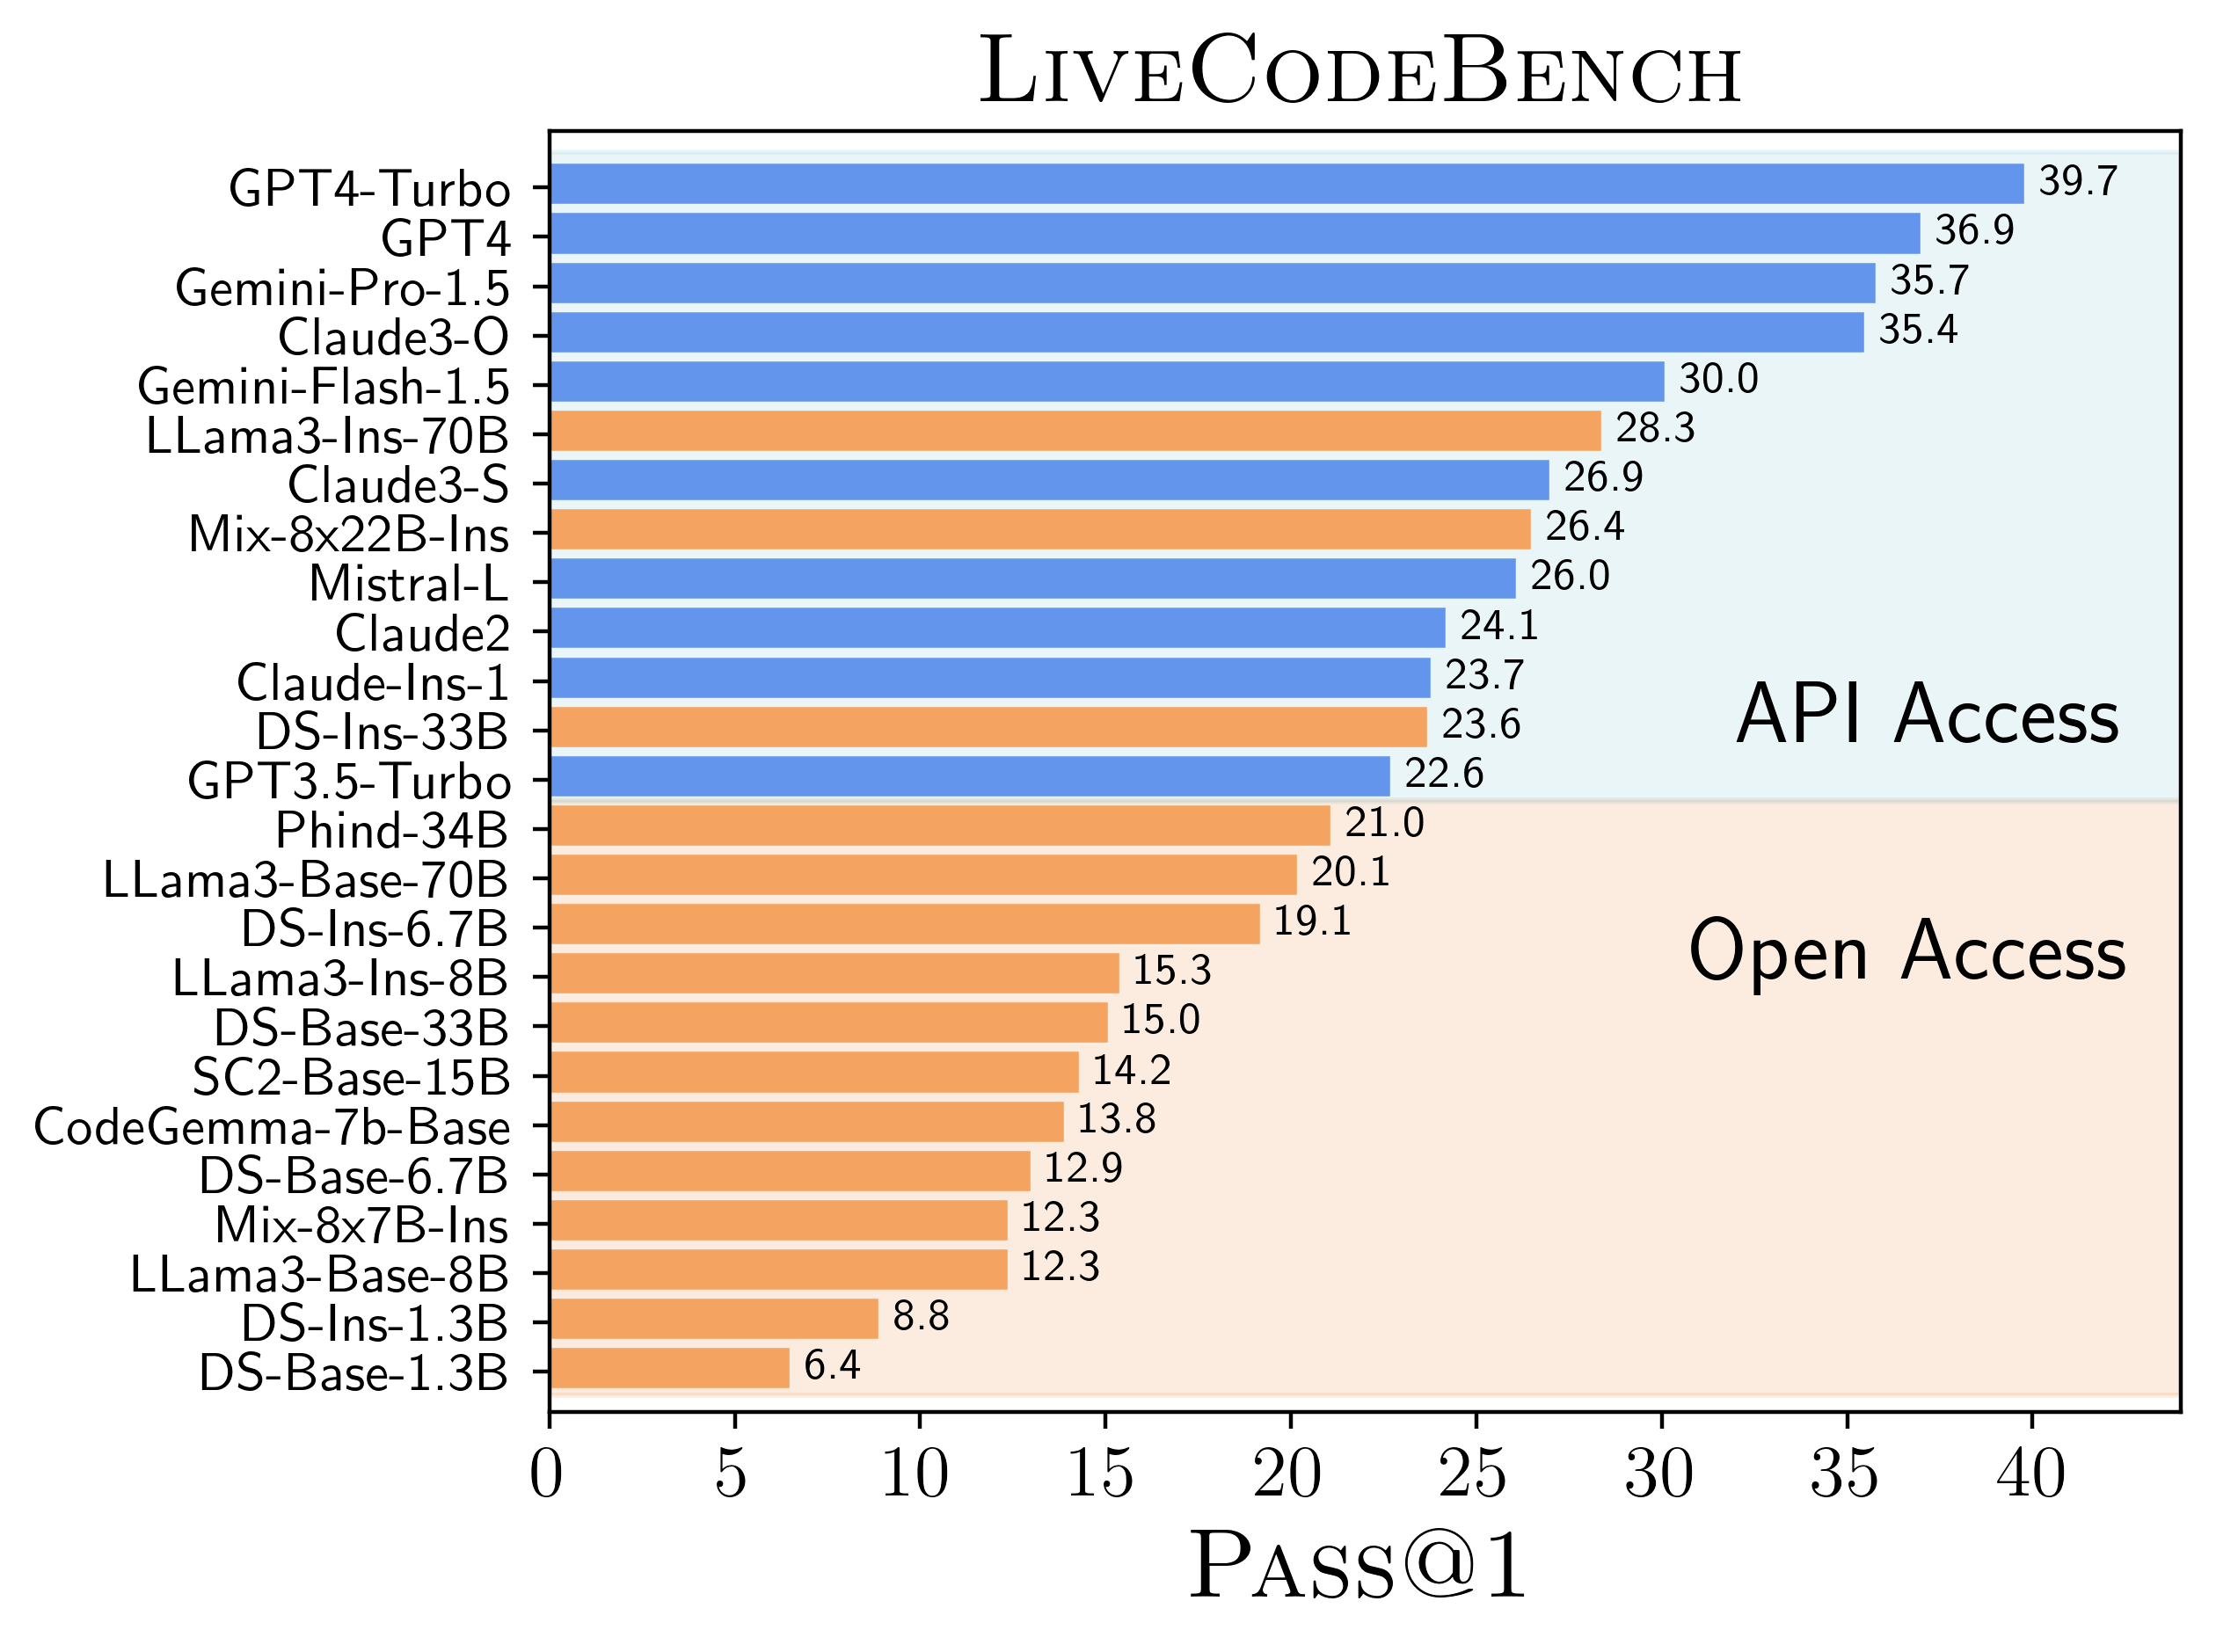
\includegraphics[width=0.65\linewidth]{figures/overview/lc_barchart.png}%

    \caption{
        Comparison of open access and (closed) API access models on \livecodebench{}
        code generation scenario. We find that closed-access models consistently 
        outperform the open models with only strong instruction-tuned variants of $>30$\textsc{B}
        models (specifically \llamaB{70}, \mixtral and  \deepseekcodeB{33} models) crossing the performance gap.
        }
    \label{fig:oss_in}
    \vspace{-10pt}
\end{figure}


\noindent \textbf{Open-Access vs Closed-Access Models.}
In general, closed (API) access model families generally outperform the open access models.
The gap is only closed by three models, namely \llamaB{70}, \mixtral{}, and \deepseekcodeB{33}
which reach the performance levels of the closed models.
For instance, in the code generation scenario (Figure~\ref{fig:oss_in}), 
these models reach close to or even outperform closed access models like \geminipro{}, \gptthreefiveturbo{}, and \claudesonnet{}.
The performances vary across scenarios with the closed-access models faring better in test output and code execution scenarios. 
%which can come close to or even outperform smaller closed models like \gptthreefiveturbo{} and \geminipro{}.
%Overall, our findings confirm that a combination of strong base models and high-quality post-training datasets is a viable recipe for good code \llms{}. 
%At the same time, we also find a lack of diverse fine-tuning
%\ag{same comment as before, ds-ins-6.7b is pretty close}


%Good instruction-tuned variants of these models (\deepseekcodeB{33} and \phind{}) can come close to or outperform various closed models. Thus, a combination of strong base models and good fine-tuning datasets allows building good code \llms{}.
%We find that fine-tuned models of both \cllamas{} and \deepseeks{} series can outperform various closed access models 

% 
% \noindent \textbf{Comparing closed models.}
% We also evaluate a range of closed models that have API access.
% The performance order remains consistent across scenarios and looks as follows: \gptfourturbo{} $>$ \gptfour{} $>$ \claudetwo{} $>$ \gptthreefiveturbo{} $~$ \geminipro{} $~$ \claudeinstantone{}.
%Among them \gptfour{} class models are significantly stronger followed by \claudetwo{}, \gptthreefiveturbo{} and \geminipro{} models in that order.

% \textbf{Comparing other open models.}
% We compare three classes of open access models, namely \deepseekcode{}, \cllama{} and \mixtral{} across different model scales. 
% First as expected, we find performance improves with model scale.
% Next, across different model classes, after considering data contamination we find that \deepseekcode{} models are significantly better than both \cllama{} and \mixtral{} models across all scenarios and the only model which consistently outperforms closed model baselines.


\textbf{Highlighting gap between SoTA}
One distinct observation from our evaluations is the large gap between SoTA models and open models across all scenarios.
Particularly, \gptfourturbo{}, \gptfour{}, \geminiproonefive{} and \claudeopus{} lead across the benchmarks with wide performance margins over other models.
This distinguishes \livecodebench{} from prior benchmarks (like \humaneval{}) where various open models have achieved similar or better performance. 
For example, \deepseekcodeB{33} is merely $4.3$ point behind \gptfourturbo{} on \humanevalplus{} but 
$16.2$ points ($69$\%) on \lcb{} code generation scenario.
This gap either holds or sometimes even amplifies across other scenarios.
%For instance, on test output prediction and code execution \gptfourturbo{} leads the \deepseekcodeB{33} model by $96\%$ and $134\%$ respectively!
%This gap is only amplified by \gptfourturbo{} which further improves over \gptfour{} across all tasks (only with \chainot{} for code execution). 
%\ag{could say a bit more for the other tasks}

% We qualitatively analyze code samples generated by the leading model, \gptfourturbo{}, and find that it generates more readable code.
% Specifically, the code consists of more inline natural language comments that \textit{reason} or \textit{plan} before producing the code.

\noindent \textbf{Comparing open-access instruction-tuned models.}
Here, we compare various fine-tuned variants of the \llamabase{}, \deepseek{} and \cllama{} base models across different model sizes.
We find that fine-tuned \llamabase{} and \deepseek{} models lead in performance, followed by \phind{} and \cllama{} models across most scenarios.
Broadly, we find that model performances correlate with model sizes. For example, \phind{} model outperforms the $6.7$\smalltextsc{B} models across all scenarios.% \nj{add llama3}

